\textbf{Use Cases 1 og 2}

Disse Use Cases beskriver følgende funktionalitet:
\begin{itemize}
	\item Gennemfør salg
	\item Returner vare
\end{itemize}
Funktionaliteten til disse Use Cases ligner hinanden. Når \gls{Eks} har udført de nødvendige
handlinger i \gls{KA} \gls{GUI} og trykker på knappen til at afslutte handel, så bliver der sendt data til \gls{CS}.

Når ekspedienten har gennemført et salg/retur i \gls{KA} så vil følgende
handlinger blive udført i systemet:
\begin{itemize}
	\item \gls{KA} opretter det korrekte kommando objekt, via \gls{SL}, med informationerne for handlen
	\item \gls{KA} bruger \gls{SL} til at konvertere kommando objektet til en XML streng
	\item XML strengen sendes til \gls{CS}
	\item \gls{CS} modtager strengen og konverterer den tilbage til den oprindelige kommando, igen ved hjælp af \gls{SL}
	\item \gls{CS} udfører de nødvendige handlinger på \gls{DB}
\end{itemize}

\begin{figure}[H]
	\centering
	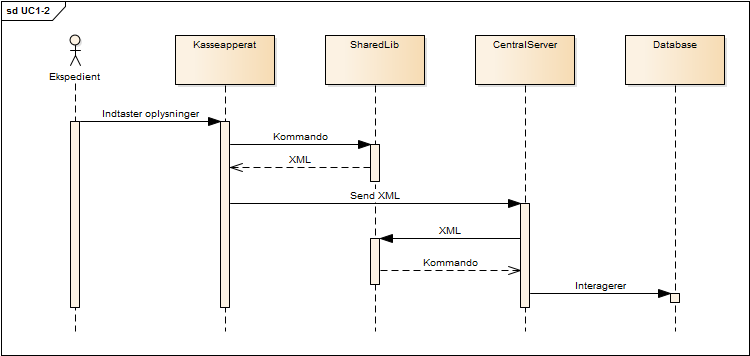
\includegraphics[width=0.8\textwidth]{Systemarkitektur/LogiskView/Realiseringer/Images/UC12.png}
	\caption{Sekvensdiagram for realisering af Use Cases 1 og 2}
	\label{fig:uc38sq}
\end{figure}

